
% Say what the application is
In this analysis dijet tracks are being clustered according to 
their $L_{xy}^\text{exp}$ as described in Section \ref{subsec:Clusters}.

Hierarchical clustering connects elements of an unclustered set using a linkage criterion
as shown schematically in Figure \ref{fig:dendrogram}.
\begin{figure}[htbp]
\centering
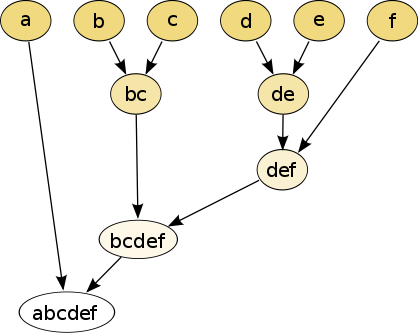
\includegraphics[width=0.5\textwidth]{plots/dendrogram.png}
% correct the plot
\caption{Dendrogram presenting hierarchical clustering. \label{fig:dendrogram}}
\end{figure}

 Initially each element is its own cluster. Each of the next steps merges exactly one pair of clusters 
with the best linkage criterion. In case of clustering numbers the linkage criterion is the minimal distance 
between clusters:

\[
\min \{\, d(x,y) : x \in \mathcal{A},\, y \in \mathcal{B} \,\}, \hspace{5pt} d(x,y)=|x-y| 
\]   

where $\mathcal{A}$ and $\mathcal{B}$ are already existing clusters. 
The procedure repeats until all elements end up
in the final cluster.   
